\vspace*{4cm}
\part{Messresultate Mesh Benchmark}\label{part:MessresultateMeshBenchmark}
\vspace*{\fill}
\clearpage

\section{Messresultate}\label{sec:Messresultate}
Bei der Durchführung der Messungen innerhalb des Mesh Benchmarks wurde für jede Messung unter den entsprechenden Bedingungen, die in der Tabelle \ref{tab:MessungenMeshBenchmark} nochmals zusammengefasst sind, ein Messprotokoll resp. eine Auswertung erstellt. Diese detaillierten Auswertungen sind im Anhang \ref{app:MessprotokolleMeshBenchmark} dem Bericht angefügt.
Nachfolgend soll exemplarisch eine dieser Auswertungen erläutert werden um aufzuzeigen was diese darstellen und wie diese gelesen werden können.

\begin{table}[h]
\centering
\begin{tabular}{|c|c|c|c|c|c|} 
\hline
\textbf{\#}  & \textbf{Msg. Gen.}  & \textbf{Duration}  & \textbf{Msg. Cnt.}  & \textbf{Payload }  & \textbf{Disturbance}  \\ 
\hline
1 & Rand & 600s & 60 & Small & No \\ 
\hline
2 & Seq & 600s & 60 & Small & No \\ 
\hline
3 & Rand & 600s & 60 & Large & No \\ 
\hline
4 & Seq & 600s & 60 & Large & No \\ 
\hline
5 & Rand & 600s & 600 & Small & No \\ 
\hline
6 & Rand & 600s & 60 & Small & Yes \\ 
\hline
7 & Seq & 750s & 10 & Small & No \\ 
\hline
8 & Seq & 750s & 10 & Large & No \\
\hline
\end{tabular}
\caption{Messungen Mesh Benchmark}
\label{tab:MessungenMeshBenchmark}
\end{table}


\subsection{Resultate}\label{subsec:Resultate}


Die Messresultate welche ausführlich im Anhang \ref{app:MessprotokolleMeshBenchmark} zu finden sind wurden mit den Messindizes 1-8 gemäss Tabelle \ref{tab:tab:MessungenMeshBenchmark} versehen um diese eindeutig identifizieren zu können.
Gemäss den Erläuterungen im Abschnitt \ref{subsec:Messreihe} wurden nicht alle Messungen in allen Messumgebungen durchgeführt.

\begin{figure}[h]
	\centering
	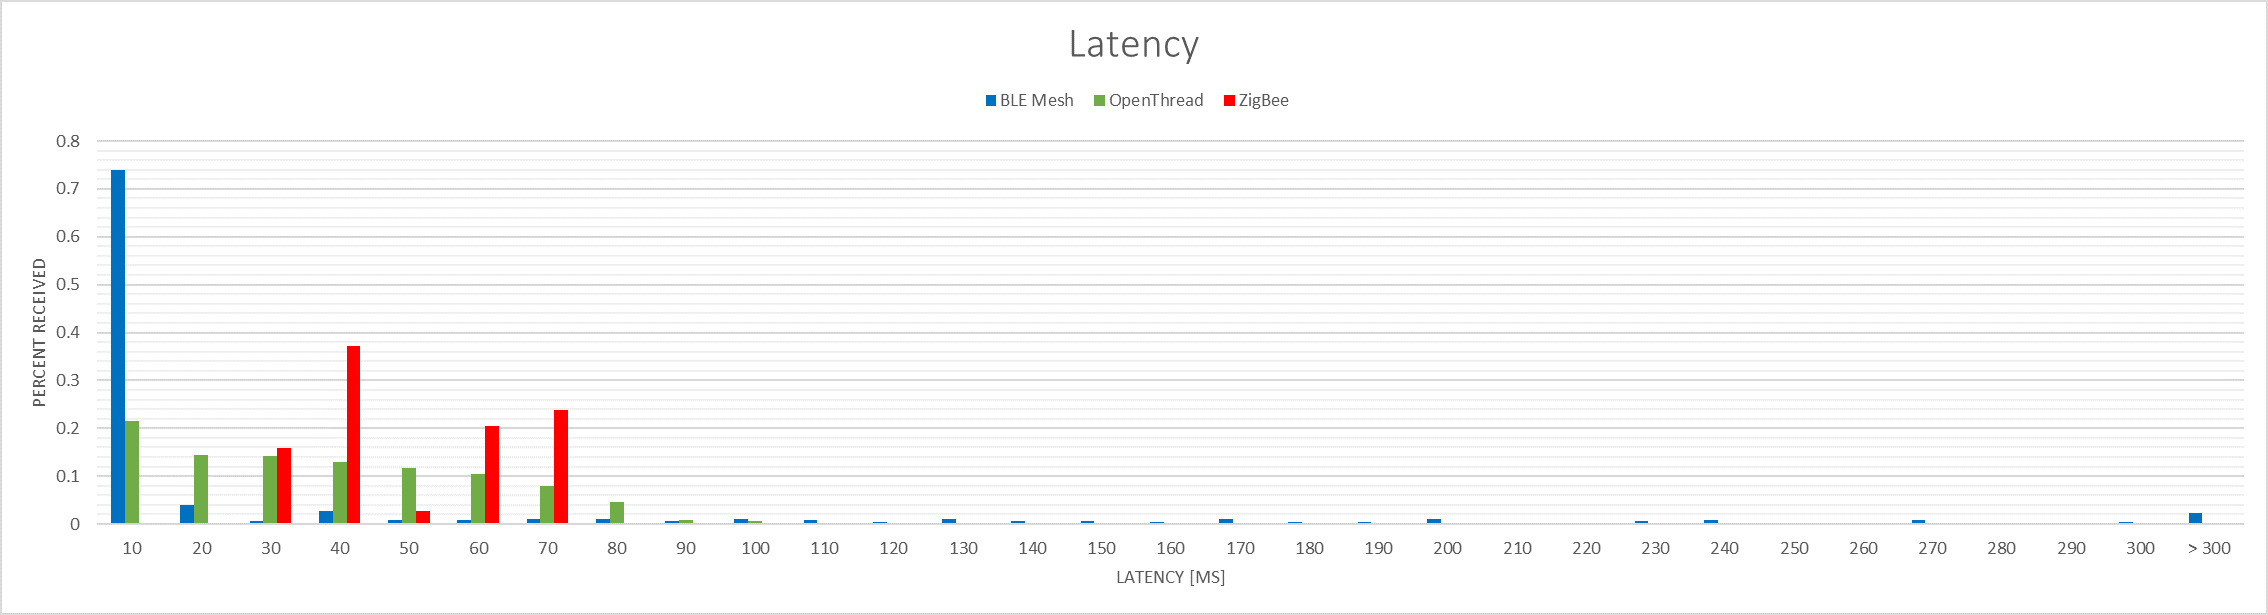
\includegraphics[width=\textwidth]{Latency_2_Wohnung.png}
	\caption{Messung 2 Wohnung: Verteilung der Latenzzeiten pro Hop}
	\label{fig:VerteilungderLatenzzeiten}
\end{figure}

Die Abbildungen \ref{fig:VerteilungderLatenzzeiten} bis \ref{fig:DurchschnittlicherEnergieverbrauch} zeigen die Messresultate der Messung 2 in der Messumgebung \textit{Wohnung}. Sie stehen exemplarisch für die Messergebnisse aller Messreihen.
In Abbildung \ref{fig:VerteilungderLatenzzeiten} ist die prozentuale Verteilung der Latenzzeiten pro Hop der drei Mesh Protokolle dargestellt.
Sie sagt also aus wie viele Nachrichten von allen angekommenen Nachrichten, das Ziel mit einer bestimmten Latenzzeit erreicht haben.
In diesem Beispiel haben rund 76 Prozent der Nachrichten die im BT Mesh Test versendet wurden das Ziel mit einer maximalen Latenzzeit von 10 Millisekunden erreicht.
Die weitere Verteilung geht bis auf Latenzzeiten von über 300 Millisekunden wobei die Prozentzahl der Nachrichten in diesem Bereich sehr tief ist.

Aus den in Abbildung \ref{fig:VerteilungderLatenzzeiten} aufgezeigten Latenzzeiten wurde in der Abbildung \ref{fig:DurchschnittlicheLatenzzeit} der Durchschnitt gebildet. Es handelt sich dabei wiederum um die Latenzzeit pro Hop. Im Falle von Zigbee ist dies erwähnenswert, da hier die Anzahl Hops nicht ausgelesen werden konnte (siehe Abschnitt \ref{subsubsec:AnzahlHops}) und die Resultate somit mit Vorsicht interpretiert werden müssen. Mehr dazu in der Validierung im Abschnitt \ref{subsec:Validierung}.

Der durchschnittliche Datendurchsatz der mit der Abbildung \ref{fig:DurchschnittlicherDurchsatz} aufgezeigt wird, muss mit der selben Vorsicht betrachtet werden. Denn auch hier werden die Werte pro Hop für die Berechnung verwendet.
Diese Werte werden errechnet aus der Paketgrösse (Small oder Large) gemäss den Definitionen in Abschnitt \ref{subsec:AllgemeineBenchmarkParameter} und der Latenzzeit des übertragenen Pakets.


\begin{figure}[!htbp]
\centering
\begin{minipage}[b]{0.49\textwidth}
		\centering
		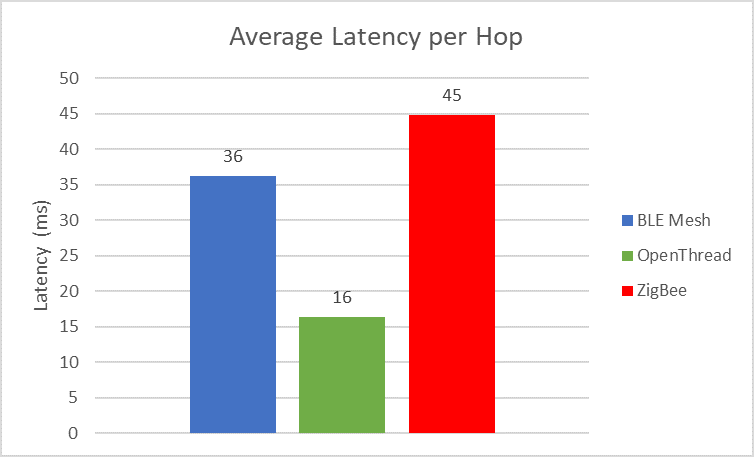
\includegraphics[width=\textwidth]{Average_Latency_per_Hop.png}
		\caption{Messung 2 Wohnung: Durchschnittliche Latenzzeit pro Hop}
		\label{fig:DurchschnittlicheLatenzzeit}
\end{minipage}
\begin{minipage}[b]{0.49\textwidth}
		\centering
		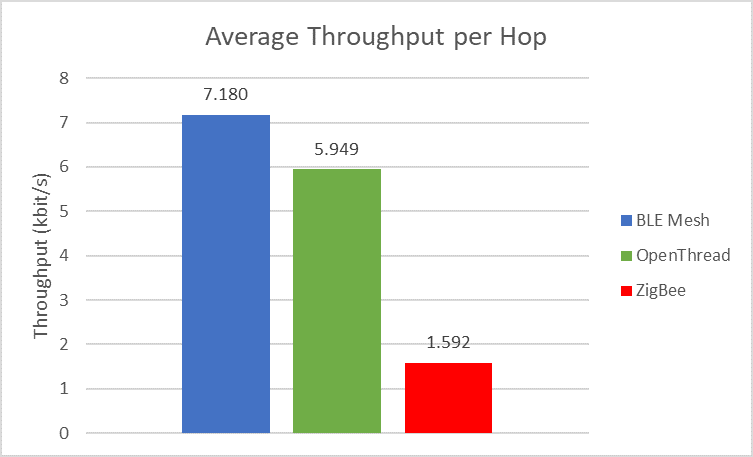
\includegraphics[width=\textwidth]{Average_Throughput_per_Hop.png}
		\caption{Messung 2 Wohnung: Durchschnittlicher Durchsatz pro Hop}
		\label{fig:DurchschnittlicherDurchsatz}
\end{minipage}
\end{figure}

In der Abbildung \ref{fig:DurchschnittlicherPaketverlust} wird der prozentuale Paketverlust gezeigt über die gesamte Anzahl Nachrichten die während dem Benchmark versendet wurden. Die Paketverluste von einzelnen Client-Server Beziehungen werden nicht separat ausgewertet.
Wiederum im Beispiel von BT Mesh sind in dieser Messung 2.07 \% der Pakete nicht am Ziel angekommen.
Zuletzt wird mit dem Diagramm in Abbildung \ref{fig:DurchschnittlicherEnergieverbrauch} der durchschnittliche Energieverbrauch der Protokolle dargestellt.
Der Energieverbrauch wurde abgeleitet aus der Aktivzeit des Funkmoduls. Diese wurde verrechnet mit dem Strombedarf des nRF52840 SoC's gemäss den Angaben in der Tabelle \ref{tab:EigenschaftennRF52840SoC}. Eine solche Berechnung erlaubt einen qualitativen Vergleich des Energiebedarf unter den 3 Protokollen da diese auf der gleichen Hardware umgesetzt wurden. Die Werte in der Abbildung \ref{fig:DurchschnittlicherEnergieverbrauch} sind jedoch keine tatsächlichen Verbrauchswerte und können deshalb nur im Kontext des Vergleichs verwendet werden.


\begin{figure}[!htbp]
\centering
\begin{minipage}[b]{0.49\textwidth}
		\centering
		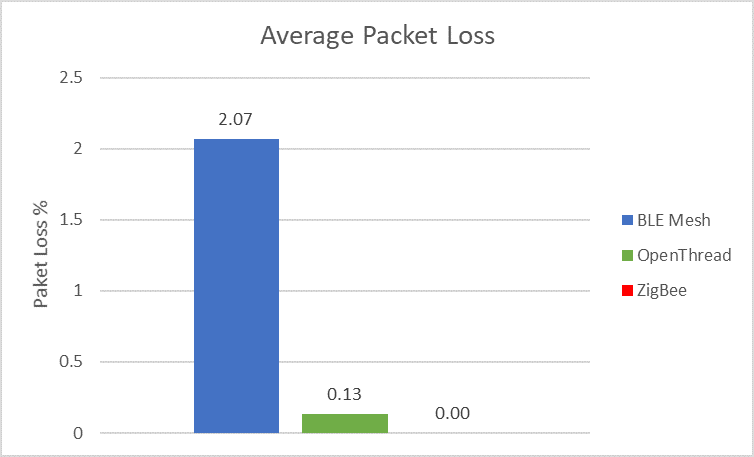
\includegraphics[width=\textwidth]{Average_Packet_Loss.png}
		\caption{Messung 2 Wohnung: Durchschnittlicher Paketverlust}
		\label{fig:DurchschnittlicherPaketverlust}
\end{minipage}
\begin{minipage}[b]{0.49\textwidth}
		\centering
		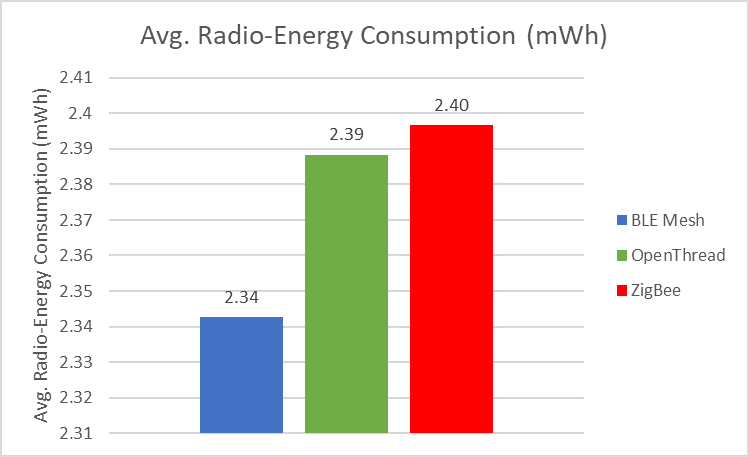
\includegraphics[width=\textwidth]{Average_Radio_Energy_Consumption.png}
		\caption{Messung 2 Wohnung: Durchschnittlicher Energieverbrauch}
		\label{fig:DurchschnittlicherEnergieverbrauch}
\end{minipage}
\end{figure}


\subsection{Validierung}\label{subsec:Validierung}


\todo[inline]{Überprüfung des eigenen Vorgehen usw.}
\todo[inline]{Fehler in Latency Zigbee da Number of Hops nicht ausgelesen werden kann.}

\begin{itemize}
\item Resultate bei grosser Payload nicht korrekt bei BT Mesh -> Überforderung des Stacks.

\item Fehler in Latency Zigbee da Number of Hops nicht ausgelesen werden kann.

\item Latency Fehler bei Zigbee kann aus der Grafik herausgelesen werden. Es gibt zwei Hauptsäulen bei 30ms und eine bei 60ms.

\item Message Dichte zu Beginn zu hoch gewählt. Darum zusätzliche Messungen 7 und 8. Zuvor unfair für BT Mesh. -> Kein hoher Durchsatz möglich.

\item Durchschnittliche Werte beinhalten Ausreisser welche das Resultat verfälschen. -> Evtl. Median bilden.

\item Packetloss: IEEE 802.15.4 hat ein MAC ACK bei Unicast Messages. Im Multicast oder Broadcast hingegen nicht. Vorteil Zigbee da Unicast Adressierung.

\item BT Mesh hat gar kein ACK. Auch nicht auf MAC Layer.

\end{itemize}

\subsection{Verifizierung}\label{subsec:Verifizierung}

\todo[inline]{Silabs Bericht}




